% Created by tikzDevice version 0.8.1 on 2015-05-24 13:12:08
% !TEX encoding = UTF-8 Unicode
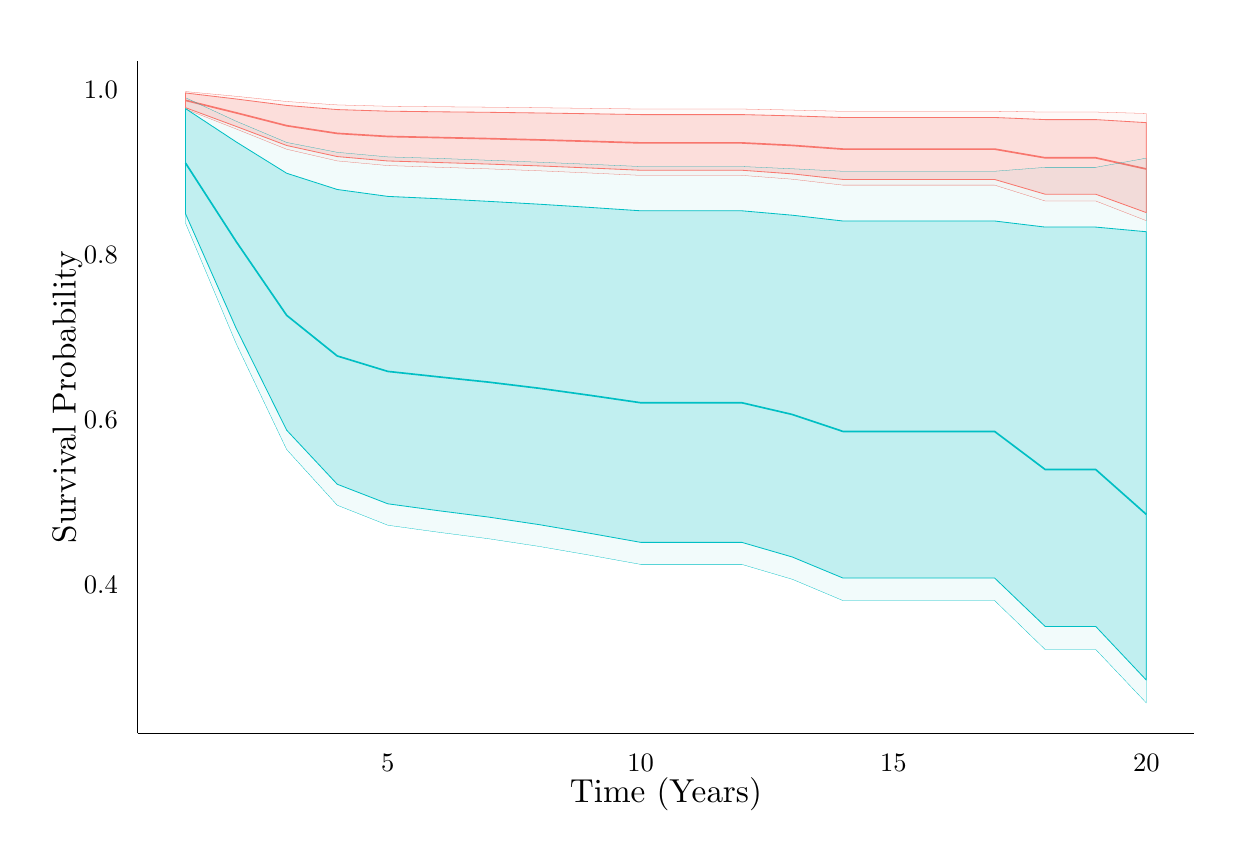
\begin{tikzpicture}[x=1pt,y=1pt]
\definecolor{fillColor}{RGB}{255,255,255}
\path[use as bounding box,fill=fillColor,fill opacity=0.00] (0,0) rectangle (433.62,289.08);
\begin{scope}
\path[clip] (  0.00,  0.00) rectangle (433.62,289.08);
\definecolor{drawColor}{RGB}{255,255,255}
\definecolor{fillColor}{RGB}{255,255,255}

\path[draw=drawColor,line width= 0.6pt,line join=round,line cap=round,fill=fillColor] (  0.00,  0.00) rectangle (433.62,289.08);
\end{scope}
\begin{scope}
\path[clip] ( 39.69, 34.03) rectangle (421.57,277.03);
\definecolor{fillColor}{RGB}{255,255,255}

\path[fill=fillColor] ( 39.69, 34.03) rectangle (421.58,277.03);
\definecolor{drawColor}{RGB}{248,118,109}

\path[draw=drawColor,line width= 0.6pt,line join=round] ( 57.05,262.81) --
	( 75.32,258.31) --
	( 93.59,253.65) --
	(111.86,250.87) --
	(130.13,249.76) --
	(148.41,249.37) --
	(166.68,248.98) --
	(184.95,248.52) --
	(203.22,248.00) --
	(221.49,247.44) --
	(239.77,247.44) --
	(258.04,247.44) --
	(276.31,246.53) --
	(294.58,245.20) --
	(312.86,245.20) --
	(331.13,245.20) --
	(349.40,245.20) --
	(367.67,242.05) --
	(385.94,242.05) --
	(404.22,238.01);
\definecolor{drawColor}{RGB}{0,191,196}

\path[draw=drawColor,line width= 0.6pt,line join=round] ( 57.05,240.14) --
	( 75.32,211.82) --
	( 93.59,185.13) --
	(111.86,170.45) --
	(130.13,164.87) --
	(148.41,162.90) --
	(166.68,160.98) --
	(184.95,158.76) --
	(203.22,156.22) --
	(221.49,153.55) --
	(239.77,153.55) --
	(258.04,153.55) --
	(276.31,149.30) --
	(294.58,143.18) --
	(312.86,143.18) --
	(331.13,143.18) --
	(349.40,143.18) --
	(367.67,129.42) --
	(385.94,129.42) --
	(404.22,113.20);
\definecolor{drawColor}{RGB}{248,118,109}
\definecolor{fillColor}{RGB}{248,118,109}

\path[draw=drawColor,line width= 0.1pt,line join=round,line cap=round,fill=fillColor,fill opacity=0.05] ( 57.05,265.99) --
	( 75.32,264.28) --
	( 93.59,262.40) --
	(111.86,261.17) --
	(130.13,260.68) --
	(148.41,260.50) --
	(166.68,260.35) --
	(184.95,260.15) --
	(203.22,259.92) --
	(221.49,259.68) --
	(239.77,259.68) --
	(258.04,259.68) --
	(276.31,259.30) --
	(294.58,258.86) --
	(312.86,258.86) --
	(331.13,258.86) --
	(349.40,258.86) --
	(367.67,258.59) --
	(385.94,258.59) --
	(404.22,258.08) --
	(404.22,219.33) --
	(385.94,226.45) --
	(367.67,226.45) --
	(349.40,232.18) --
	(331.13,232.18) --
	(312.86,232.18) --
	(294.58,232.18) --
	(276.31,234.32) --
	(258.04,235.71) --
	(239.77,235.71) --
	(221.49,235.71) --
	(203.22,236.56) --
	(184.95,237.36) --
	(166.68,238.05) --
	(148.41,238.65) --
	(130.13,239.25) --
	(111.86,240.93) --
	( 93.59,245.15) --
	( 75.32,252.47) --
	( 57.05,259.66) --
	cycle;
\definecolor{drawColor}{RGB}{0,191,196}
\definecolor{fillColor}{RGB}{0,191,196}

\path[draw=drawColor,line width= 0.1pt,line join=round,line cap=round,fill=fillColor,fill opacity=0.05] ( 57.05,263.76) --
	( 75.32,255.28) --
	( 93.59,247.61) --
	(111.86,244.04) --
	(130.13,242.38) --
	(148.41,241.84) --
	(166.68,241.16) --
	(184.95,240.46) --
	(203.22,239.70) --
	(221.49,238.91) --
	(239.77,238.91) --
	(258.04,238.91) --
	(276.31,238.09) --
	(294.58,237.19) --
	(312.86,237.19) --
	(331.13,237.19) --
	(349.40,237.19) --
	(367.67,238.60) --
	(385.94,238.60) --
	(404.22,241.93) --
	(404.22, 45.08) --
	(385.94, 64.38) --
	(367.67, 64.38) --
	(349.40, 82.07) --
	(331.13, 82.07) --
	(312.86, 82.07) --
	(294.58, 82.07) --
	(276.31, 89.75) --
	(258.04, 95.14) --
	(239.77, 95.14) --
	(221.49, 95.14) --
	(203.22, 98.44) --
	(184.95,101.61) --
	(166.68,104.39) --
	(148.41,106.76) --
	(130.13,109.29) --
	(111.86,116.52) --
	( 93.59,136.63) --
	( 75.32,174.95) --
	( 57.05,218.42) --
	cycle;
\definecolor{drawColor}{RGB}{248,118,109}
\definecolor{fillColor}{RGB}{248,118,109}

\path[draw=drawColor,line width= 0.3pt,line join=round,line cap=round,fill=fillColor,fill opacity=0.20] ( 57.05,265.48) --
	( 75.32,263.31) --
	( 93.59,260.98) --
	(111.86,259.48) --
	(130.13,258.90) --
	(148.41,258.68) --
	(166.68,258.49) --
	(184.95,258.25) --
	(203.22,257.97) --
	(221.49,257.67) --
	(239.77,257.67) --
	(258.04,257.67) --
	(276.31,257.21) --
	(294.58,256.62) --
	(312.86,256.62) --
	(331.13,256.62) --
	(349.40,256.62) --
	(367.67,255.86) --
	(385.94,255.86) --
	(404.22,254.76) --
	(404.22,222.25) --
	(385.94,228.89) --
	(367.67,228.89) --
	(349.40,234.23) --
	(331.13,234.23) --
	(312.86,234.23) --
	(294.58,234.23) --
	(276.31,236.25) --
	(258.04,237.56) --
	(239.77,237.56) --
	(221.49,237.56) --
	(203.22,238.37) --
	(184.95,239.12) --
	(166.68,239.78) --
	(148.41,240.35) --
	(130.13,240.91) --
	(111.86,242.50) --
	( 93.59,246.50) --
	( 75.32,253.40) --
	( 57.05,260.16) --
	cycle;
\definecolor{drawColor}{RGB}{0,191,196}
\definecolor{fillColor}{RGB}{0,191,196}

\path[draw=drawColor,line width= 0.3pt,line join=round,line cap=round,fill=fillColor,fill opacity=0.20] ( 57.05,259.83) --
	( 75.32,247.81) --
	( 93.59,236.47) --
	(111.86,230.61) --
	(130.13,228.11) --
	(148.41,227.27) --
	(166.68,226.31) --
	(184.95,225.28) --
	(203.22,224.13) --
	(221.49,222.91) --
	(239.77,222.91) --
	(258.04,222.91) --
	(276.31,221.31) --
	(294.58,219.22) --
	(312.86,219.22) --
	(331.13,219.22) --
	(349.40,219.22) --
	(367.67,217.02) --
	(385.94,217.02) --
	(404.22,215.34) --
	(404.22, 53.33) --
	(385.94, 72.71) --
	(367.67, 72.71) --
	(349.40, 90.21) --
	(331.13, 90.21) --
	(312.86, 90.21) --
	(294.58, 90.21) --
	(276.31, 97.80) --
	(258.04,103.10) --
	(239.77,103.10) --
	(221.49,103.10) --
	(203.22,106.36) --
	(184.95,109.48) --
	(166.68,112.21) --
	(148.41,114.54) --
	(130.13,117.03) --
	(111.86,124.10) --
	( 93.59,143.63) --
	( 75.32,180.48) --
	( 57.05,221.79) --
	cycle;
\end{scope}
\begin{scope}
\path[clip] (  0.00,  0.00) rectangle (433.62,289.08);
\definecolor{drawColor}{RGB}{0,0,0}

\path[draw=drawColor,line width= 0.6pt,line join=round] ( 39.69, 34.03) --
	( 39.69,277.03);
\end{scope}
\begin{scope}
\path[clip] (  0.00,  0.00) rectangle (433.62,289.08);
\definecolor{drawColor}{RGB}{0,0,0}

\node[text=drawColor,anchor=base east,inner sep=0pt, outer sep=0pt, scale=  0.96] at ( 32.57, 84.49) {0.4};

\node[text=drawColor,anchor=base east,inner sep=0pt, outer sep=0pt, scale=  0.96] at ( 32.57,144.11) {0.6};

\node[text=drawColor,anchor=base east,inner sep=0pt, outer sep=0pt, scale=  0.96] at ( 32.57,203.73) {0.8};

\node[text=drawColor,anchor=base east,inner sep=0pt, outer sep=0pt, scale=  0.96] at ( 32.57,263.36) {1.0};
\end{scope}
\begin{scope}
\path[clip] (  0.00,  0.00) rectangle (433.62,289.08);
\definecolor{drawColor}{RGB}{0,0,0}

\path[draw=drawColor,line width= 0.6pt,line join=round] ( 39.69, 34.03) --
	(421.57, 34.03);
\end{scope}
\begin{scope}
\path[clip] (  0.00,  0.00) rectangle (433.62,289.08);
\definecolor{drawColor}{RGB}{0,0,0}

\node[text=drawColor,anchor=base,inner sep=0pt, outer sep=0pt, scale=  0.96] at (130.13, 20.31) {5};

\node[text=drawColor,anchor=base,inner sep=0pt, outer sep=0pt, scale=  0.96] at (221.49, 20.31) {10};

\node[text=drawColor,anchor=base,inner sep=0pt, outer sep=0pt, scale=  0.96] at (312.86, 20.31) {15};

\node[text=drawColor,anchor=base,inner sep=0pt, outer sep=0pt, scale=  0.96] at (404.22, 20.31) {20};
\end{scope}
\begin{scope}
\path[clip] (  0.00,  0.00) rectangle (433.62,289.08);
\definecolor{drawColor}{RGB}{0,0,0}

\node[text=drawColor,anchor=base,inner sep=0pt, outer sep=0pt, scale=  1.20] at (230.63,  9.03) {Time (Years)};
\end{scope}
\begin{scope}
\path[clip] (  0.00,  0.00) rectangle (433.62,289.08);
\definecolor{drawColor}{RGB}{0,0,0}

\node[text=drawColor,rotate= 90.00,anchor=base,inner sep=0pt, outer sep=0pt, scale=  1.20] at ( 17.30,155.53) {Survival Probability};
\end{scope}
\end{tikzpicture}
